\section{长度的测量}\label{sec:1-1}

人们在建造铁路、房屋,计算土地面积的时候,都要测量长度。
测量长度,首先要确定一个标准长度,用标准长度去量被测的长度,才能得出被测长度的数值。
这个被确定的标准长度叫做\CJKunderwave{长度单位}。

世界各国原来使用的长度单位很不相同,例如,在我国用市尺,在英、美等国用英尺。
后来为了便于科学技术的交流,国际上规定了一套统一的单位,叫做\textbf{国际单位制},
已经被包括我国在内的许多国家采用。在今后学习中,我们将主要使用国际单位制。
在国际单位制中,长度的主单位是\textbf{米}(也叫公尺)。

用米作单位,北尔到哈尔滨的铁路长度大约是 1 388 000 米,这种写法数字较大;
物理课本中一张纸的厚度,大约是 0.000 075 米,这种写法数字又太小。
数字太大或太小,读和写都不方便。因此,又规定了比米大的单位和比米小的单位。
比米大的单位有千米(也叫公里),比米小的单位有分米、厘米、毫米、微米等。
它们之间的关系是
\vspace{-1em}\begin{center}
    \begin{tabular}{l}
        1 千米 = 1000 米, \\
        1  米 = 10 分米, \\
        1 分米 = 10 厘米, \\
        1 厘米 = 10 毫米, \\
        1 毫米 = 1000 微米。 \\
    \end{tabular}
\end{center}\vspace{-1em}
这样,北京到哈尔滨的铁路长度就可以用千米作单位,是 1388 千米,
而物理课本中一张纸的厚度就可以用微米作单位,是 75 微米。

\begin{figure}[htbp]
    \centering
    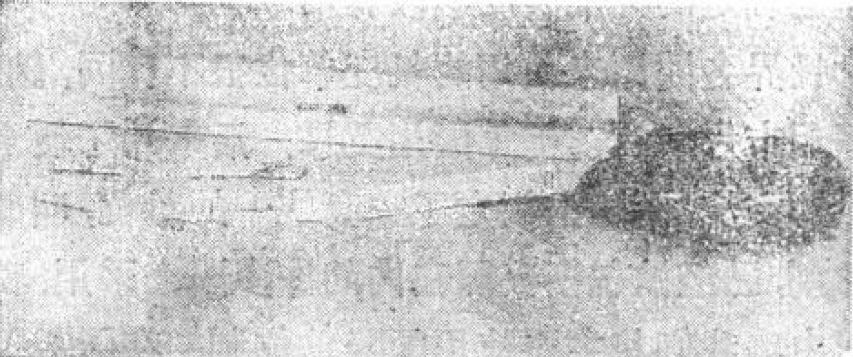
\includegraphics[width=0.5\textwidth]{../pic/czwl1-ch1-1}
    \caption{木尺,卷尺}\label{fig:1-1}
\end{figure}

测量长度的基本工具是刻度尺(图\ref{fig:1-1})。
用最小刻度是厘米的尺来测量,厘米下一位的毫米数要靠眼睛来估计,估计的数值就和真实的值有差异,所以测量只能准确到厘米。
用最小刻度是毫米的尺来测量,毫米下一位的数字要靠眼睛来估计,所以测量只能准确到毫米。
可见,\CJKunderwave{测量所能达到的准确程度是由刻度尺的最小刻度决定的}。

为了制作窗帘而测量窗户的长度,准确到厘米就足够了,为了安装玻璃而测量窗户的长度,就要准确到毫米,否则,
玻璃的大小跟窗框相差太多,就可能安装不上去。可见,\CJKunderwave{测量需要达到的准确程度跟测量的要求有关系}。

\begin{figure}[htbp]
    \centering
    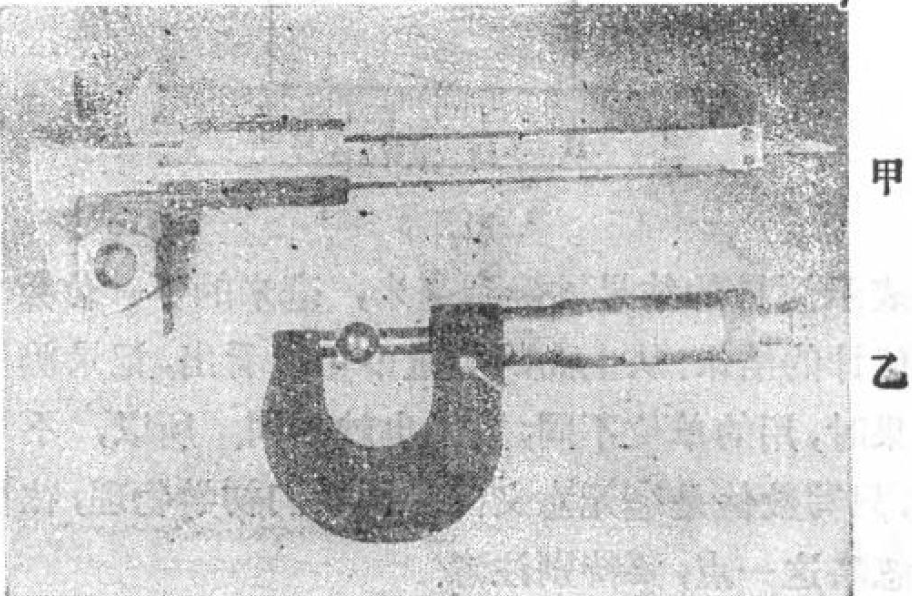
\includegraphics[width=0.5\textwidth]{../pic/czwl1-ch1-2}
    \caption{甲:游标卡尺 \hspace{1em} 乙:螺旋测微器}\label{fig:1-2}
\end{figure}

随着生产技术的发展,工业上对于某些产品或零件的测量,要求越来越严格,有时需要准确到 $0.01$ 毫米,
甚至需要准确到微米。一般最小刻度是厘米或毫米的尺就不能满足需要了,于是人们又研制出了一些精密的测量长度的工具,
游标卡尺( 图 \ref{fig:1-2} 甲) 测量的准确程度可以达到 $0.1$ 毫米、$0.05$ 毫米或 $0.02$ 毫米。
螺旋测微器,也叫千分尺( 图 \ref{fig:1-2} 乙),测量的准确程度可以达到 $0.01$ 毫米。
工厂里常常使用这两种测量工具。它们的原理和使用方法到高中将要学习。
除此以外,人们还制造出了各种光学测量仪器,用它们来测量长度,准确程度就更高了。
\CJKunderwave{在测量长度的时候,要先根据实际情况确定测量需要达到的准确程度,然后再根据要求选用适当的测量工具}。

\begin{figure}[htbp]
    \centering
    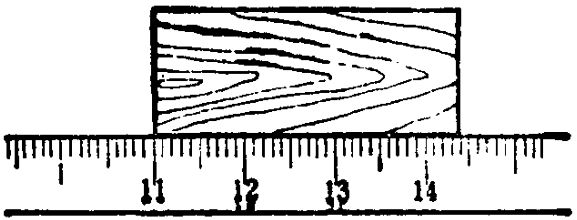
\includegraphics[width=0.5\textwidth]{../pic/czwl1-ch1-3}
    \caption{}\label{fig:1-3}
\end{figure}

\CJKunderwave{记录测量的结果,必须在数值后面写出所用的单位}。
例如,在图 \ref{fig:1-3} 所示的测量中,用的尺最小刻度是毫米,
如果用厘米作单位,木块的长度就是 $3.39$ 厘米,
如果用毫米作单位,木块的长度就是 $33.9$ 毫米。
这样写表示测量的结果准确到毫米,毫米的下一位数字 $9$ 是估计的结果。
从上面的测量中可以看出,记录测量的结果时,用的单位不同,数值也就不同。
所以,不写单位,只写数值是毫无意义的。
同学们初学物理,往往容易忽略这一点,要特别注意。

\begin{table}[H]
    \centering
    \caption*{一些距离和长度 (单位:米)}
    \begin{tabular}{w{l}{10em}w{r}{8em}}
        银河系的半径        & $6 \times 10^{19}$ \\
        太阳的半径          & $7 \times 10^8$ \\
        地球到月球的距离    & $3.8 \times 10^8$ \\
        地球的半径          & $6.4 \times 10^6$ \\
        月球的半径          & $1.7 \times 10^6$ \\
        一张纸的厚度        & $0.7 \text{~} 1 \times 10^{-4}$\footnotemark \\
        链球菌的半径        & $0.3 \text{~} 0.5 \times 10^{-6}$ \\
        原子的半径          & $0.5 \text{~} 3 \times 10^{-10}$ \\
    \end{tabular}
\end{table}
\footnotetext{$10^{-4}$ 是一种表示小数的科学记数法。这种记数法表示的意思是
$10^{-1} = 0.1$,
$10^{-2} = 0.01$,
$10^{-3} = 0.001$,…… ,
$0.7 \text{~} 1 \times 10^{-4}$ 就是 $0.00 \; 007$ ~ $0.0 \; 001$。
}


\nonumsection{阅读材料: 长度单位的发展过程}

长度的单位是可以任意规定的。从古到今,不同的国家,不同的时代,用过不同的长度单位。
古代,人们常常用身体的某些部分作为长度单位。
比如,我国古书《孔子家语》中有“布手知尺”的说法,意思是把张开的大拇指和中指两端间的距离作为 $1$ 尺。
埃及在建造金字塔的时候,曾经用肘到中指尖的距离作为长度单位。
英国曾经用从国王亨利第一的鼻尖到平伸手臂的手指尖的距离作为长度单位。
除此以外,古代还用某物品的长度作为长度单位,比如我国《汉书 \; 律历志》上记载着,以一粒黍的宽度作为 $1$ 分。
这类长度单位的缺点是长短不固定,造成测量上的混乱。

1791 年,法国决定把通过巴黎的子午线,从赤道到北极的长度的 $\dfrac{1}{10 \; 000 \; 000}$ (图 \ref{fig:1-4})作为长度单位,叫做米。
后来根据测量结果用纯铂制成了一个标准米原器,保存在法国档案局。


\begin{figure}[htbp]
    \centering
    \begin{minipage}{7cm}
    \centering
    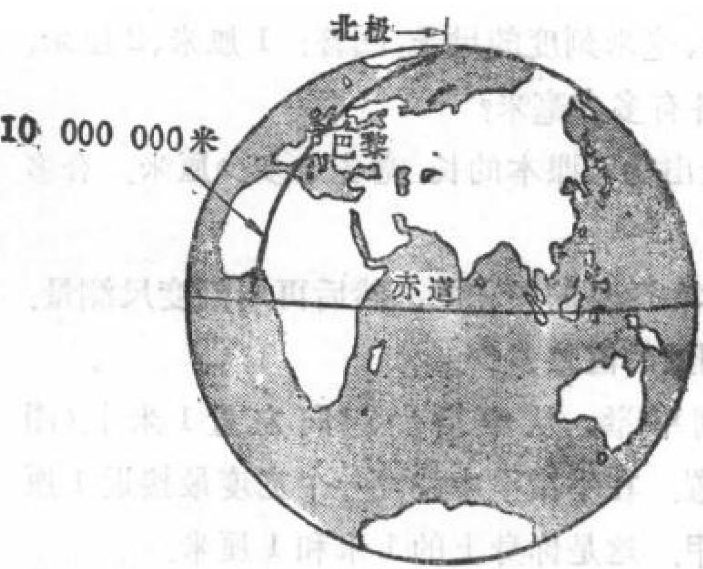
\includegraphics[width=4cm]{../pic/czwl1-ch1-4}
    \caption{}\label{fig:1-4}
    \end{minipage}
    \qquad
    \begin{minipage}{6cm}
    \centering
    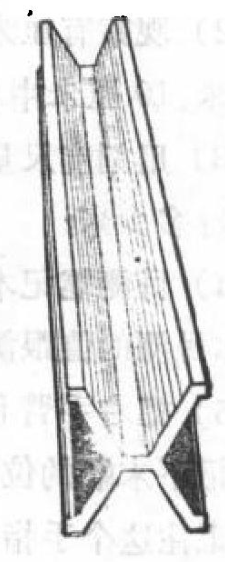
\includegraphics[width=1cm]{../pic/czwl1-ch1-5}
    \caption{国际米原器}\label{fig:1-5}
    \end{minipage}
\end{figure}


由于米的长度比较固定,优点比较多,陆续被许多国家采用。
1889 年用含 $90\%$ 的铂和 $10\%$ 的铱的合金制成了一个横截面是 X 形的国际米原器(图 \ref{fig:1-5}),
保存在法国巴黎的国际计量局里。在它的凹槽的两端分别刻着三条细线,温度是 0 ℃ 时,
两端的中间一条细线之间的距离是 $1$ 米。


用米作长度单位比用人体某些部分或某些物品作长度单位前进了一大步。但是,由于米原器天长日久会变形,
不能适应科学技术发展的更高耍求。 1960 年国际上决定用原子光谱来规定米的长度。

19 世纪 50 年代,在中法通商中米开始传入我国。现在我国已正式采用米作为长度单位。


\lianxi

(1) 在你的刻度尺上分别找出1 厘米、1 分来的长度, 并且画在作业本上。

(2) 观察有厘米、毫米刻度的尺子,回答: 1 厘米、2 厘米、$4.5$ 厘米、10 厘米中各有多少毫米?

(3) 用刻度尺量出物理课本的长、宽各是多少厘米。合多少分米? 多少米?

(4) 目测笔记本和课桌的长和宽,然后再用刻度尺测量。看看你目测的值跟测量的值差多少。

(5) 把右手臂侧平举,从中指尖起向左量 1 米长(图 \ref{fig:1-6}), 记下末端的位置。
在手指甲中找出一个宽度最接近 1 厘米的,记住这个手指甲。
这是你身上的 1 米和 1 厘米。

用你身上的 1 米测量教室的长和宽,并跟用卷尺测量的结果相比较。
用你身上的 1 厘米测量铅笔的长,并跟用刻度尺测量的结果相比较。

\begin{figure}[htbp]
    \centering
    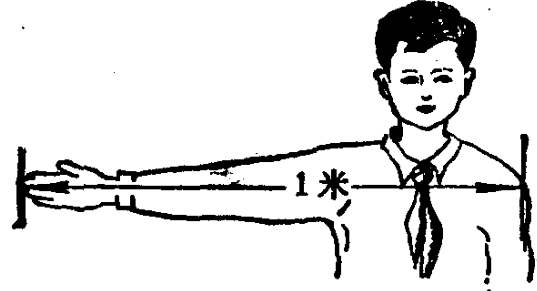
\includegraphics[width=0.3\textwidth]{../pic/czwl1-ch1-6}
    \caption{}\label{fig:1-6}
\end{figure}

(6) 人的身高早晨比晚上高。找一个人量一量,看看他早上比晚上高多少(用毫米作单位)。

(7) 地球的半径是 $6.4 \times 10^3$ 千米,合多少米?多少厘米?

(8) 地球到月球的距离是 $3.8 \times 10^8$ 米,合多少千米?

